% !TEX root = ../../main.tex

\subsection{The structural transition leading to NGA in DUT-49}

In the time-resolved pressure and calorimetry signal recorded when
performing butane adsorption at \SI{303}{\kelvin}, the NGA step 
is clearly visible as the pressure in the cell suddenly increases 
after a dosing point. An example can be seen 
in \autoref{dut:fig:dut-49-transient}, next to a regular dosing step.
A short time after the adsorbate is introduced in the measurement
cell, the material contracts. The calorimeter signal is
positive, therefore the overall process is still exothermic --- even
though desorption and structural transition, both endothermic
processes, are taking place.

\begin{figure}[htb]
    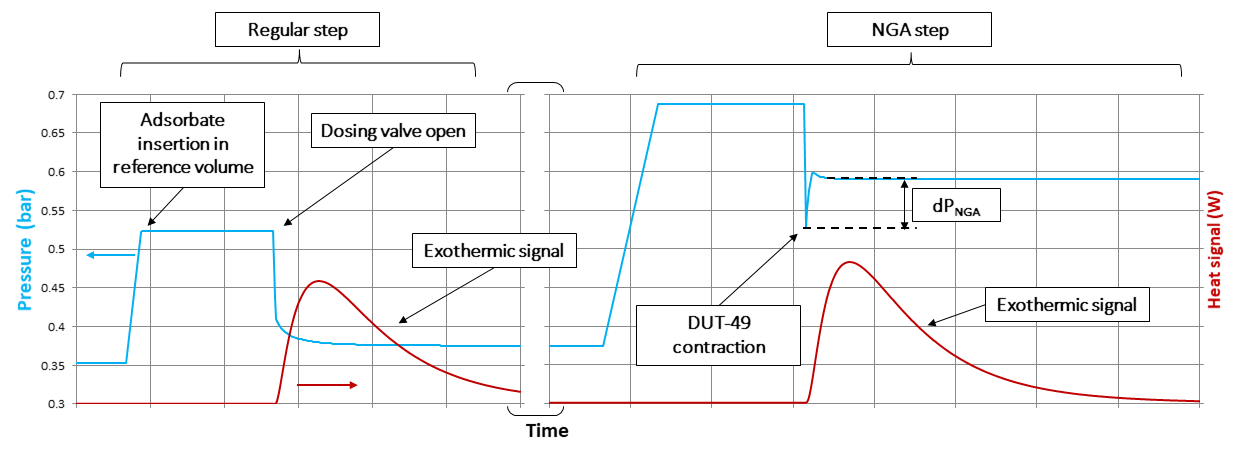
\includegraphics[width=\textwidth]{rtc/dut-49-transient}%
    \caption{The pressure and calorimeter signal from butane adsorption
    on DUT-49, highlighting a typical step (left) and the 
    observed NGA step (right)}%
    \label{dut:fig:dut-49-transient}
\end{figure}

The signals are then processed to yield the combined isotherm and
differential heat of adsorption. \autoref{dut:fig:dut-49-butane} shows
two isotherms recorded on different DUT-49 samples. 
Several observations can be made. First, a clear transition takes place
around \(0.15~p/p_0\). This corresponds to the \textit{op}/\textit{cp} 
transition which \textit{decreases} the amount adsorbed per gram 
of material. After NGA, the material is in its \textit{cp} form,
where it remains throughout the remainder of the measurement. 
Unlike in the methane experiments performed at 
\SI{111}{\kelvin}, the structure does not re-open. A secondary 
transition to the \textit{op} form is expected at higher pressures,
close to the saturation pressure of the adsorbate. However, this 
pressure range could not be reached within the experimental conditions.
\todo{Need simulated isotherms from Simon}

\begin{figure}[htb]
    \centering
    \begin{subfigure}{0.33\linewidth}
        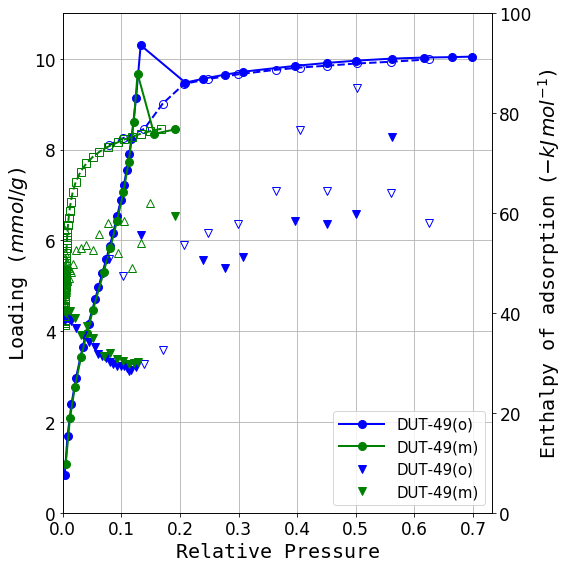
\includegraphics[width=\linewidth]{rtc/dut-49-butane-reg}%
        \caption{}\label{dut:fig:dut-49-butane-reg}
    \end{subfigure}%
    \begin{subfigure}{0.33\linewidth}
        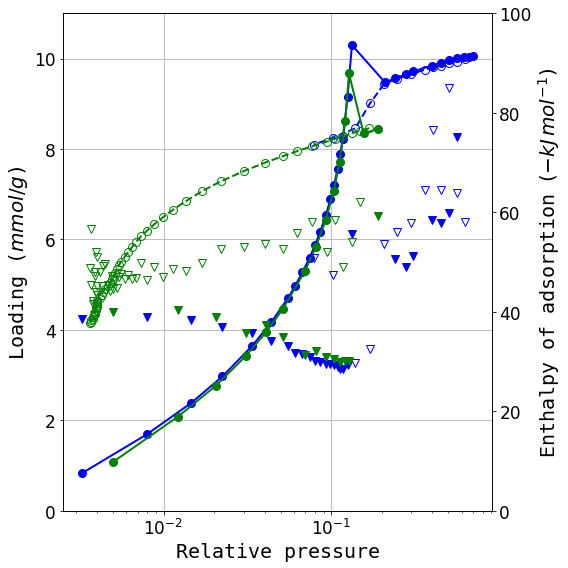
\includegraphics[width=\linewidth]{rtc/dut-49-butane-log}%
        \caption{}\label{dut:fig:dut-49-butane-log}
    \end{subfigure}%
    \begin{subfigure}{0.33\linewidth}
        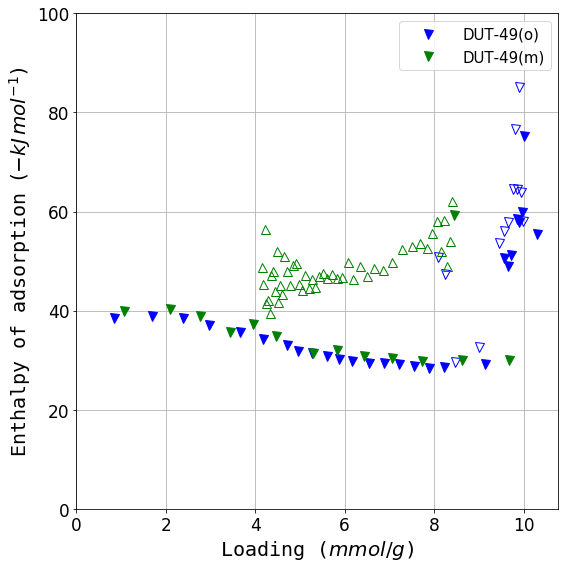
\includegraphics[width=\linewidth]{rtc/dut-49-butane-enth}%
        \caption{}\label{dut:fig:dut-49-butane-enth}
    \end{subfigure}%
    \caption{Butane adsorption experiments on two samples of 
    DUT-49, DUT-49(o) and DUT-49(m) shown as (a) regular 
    isotherms (b) logarithmic isotherms 
    and (c) enthalpy as a function of pressure.}%
    \label{dut:fig:dut-49-butane}
\end{figure}

Due to the steep knee in the adsorption/desorption branch of the 
\textit{cp} form, a complete desorption branch cannot be obtained,
with the minimum attained loading of \SI{4}{\milli\mol}. As such,
framework collapse is not seen in the experiments. Another 
shortcoming is that the isotherm
and energy landscape of the \textit{op} form in its metastable 
region is inaccessible, since by definition the material will 
undergo a transition in this pressure range.

A key feature visible in the two recorded isotherms is that,
while adsorption on the open pore form fully overlaps between the 
two experiments, both the location and extent of NGA differ 
slightly. In the DUT-49(o) isotherm, a smaller NGA step occurs,
with the resulting structural contraction apparently unable to 
achieve a complete closing of the pores. Upon desorption, a 
secondary step occurs in the same \(0.15-0.2~p/p_0\) pressure range,
after which the material is fully in its \textit{cp} state,
as evidenced by the overlap with the DUT-49(m) isotherm. The 
reason behind the dissimilar behaviour is the contribution
of crystal size to the energy barrier of transition. A thorough
analysis can be found in the paper published 
by \citet{krauseEffectCrystalliteSize2018} where it shown that 
a high surface to volume ratio has a negative impact on NGA, with 
smaller crystallites unable to achieve a complete contraction,
instead accessing an intermediated or \textit{ip}, with the \textit{``a''}
lattice parameter 5--7\% smaller than the \textit{op} phase
rather than 24\% in the \textit{cp} phase.

The enthalpy curves in \autoref{dut:fig:dut-49-butane-enth},
paint a picture of the energetic landscape of both phases.
First it should be noted that the differential enthalpy of
the NGA step itself does not appear on the graph as it is a
negative value. This is not because the transition step is 
endothermic, as proven in \autoref{dut:fig:dut-49-transient}. 
However, as the net change in adsorbed amount between the two
points where the transition occurs is negative, the calculated
enthalpy \textit{per mol of gas adsorbed} takes the same sign.

In the adsorption branch, the initial enthalpy of adsorption 
can be observed to be around \SIrange{38}{40}{\kilo\joule\per\mol}.
This value is relatively low for a copper-based 
MOF~\cite{langeStructuralFlexibilityCopperbased2014} and suggest
that the interaction of the pore wall with the adsorbate is 
relatively low. After \SI{2}{\milli\mol\per\gram}, the enthalpy
curve slopes downwards until a local minima around 
\SI{30}{\kilo\joule\per\mol} before NGA. 
This is the multilayer adsorption region,
where the field gradient of the pore wall decreases and guest-guest 
interactions dominate.
The enthalpy calculated for the desorption curve is essentially the 
differential enthalpy of adsorption on the \textit{cp} form. A large 
difference, in the range of \SIrange{10}{20}{\kilo\joule\per\mol}, exists
between the enthalpy of adsorption in the two states. This can be 
attributed to the microporous nature of the \textit{cp} form, with the
smaller pore walls increasing the interaction of the framework backbone
with an adsorbate molecule. The energy required to drive the 
transition and generate the observed thermal effect can be accounted 
for by the increased total interactions of remaining adsorbed 
molecules with the \textit{cp} state of the framework.
A more in-depth analysis of the NGA energetics will be presented 
in \autoref{dut:indepth}.

\subsubsection{A brief analysis of measurement uncertainty}

In order to assess whether results obtained through calorimetry
are within acceptable accuracy, uncertainty calculations have been
carried out. The method used here is laid out by the International 
Organisation for Standardisation (ISO) in the Guide to the expression
of Uncertainty in Measurements (GUM). The method is fully detailed 
in \autoref{appx:errors}, and consists of an identification of 
all variables used in the calculation of the final result, and 
estimation of the uncertainty in the final value as a function of
the uncertainty in each such variable. The result is multiplied
by a factor of confidence, which has been chosen as 95\% in the 
figures presented in \autoref{dut:fig:dut-49-butane-err}.


\begin{figure}[htb]
    \centering
    \begin{subfigure}{0.33\linewidth}
        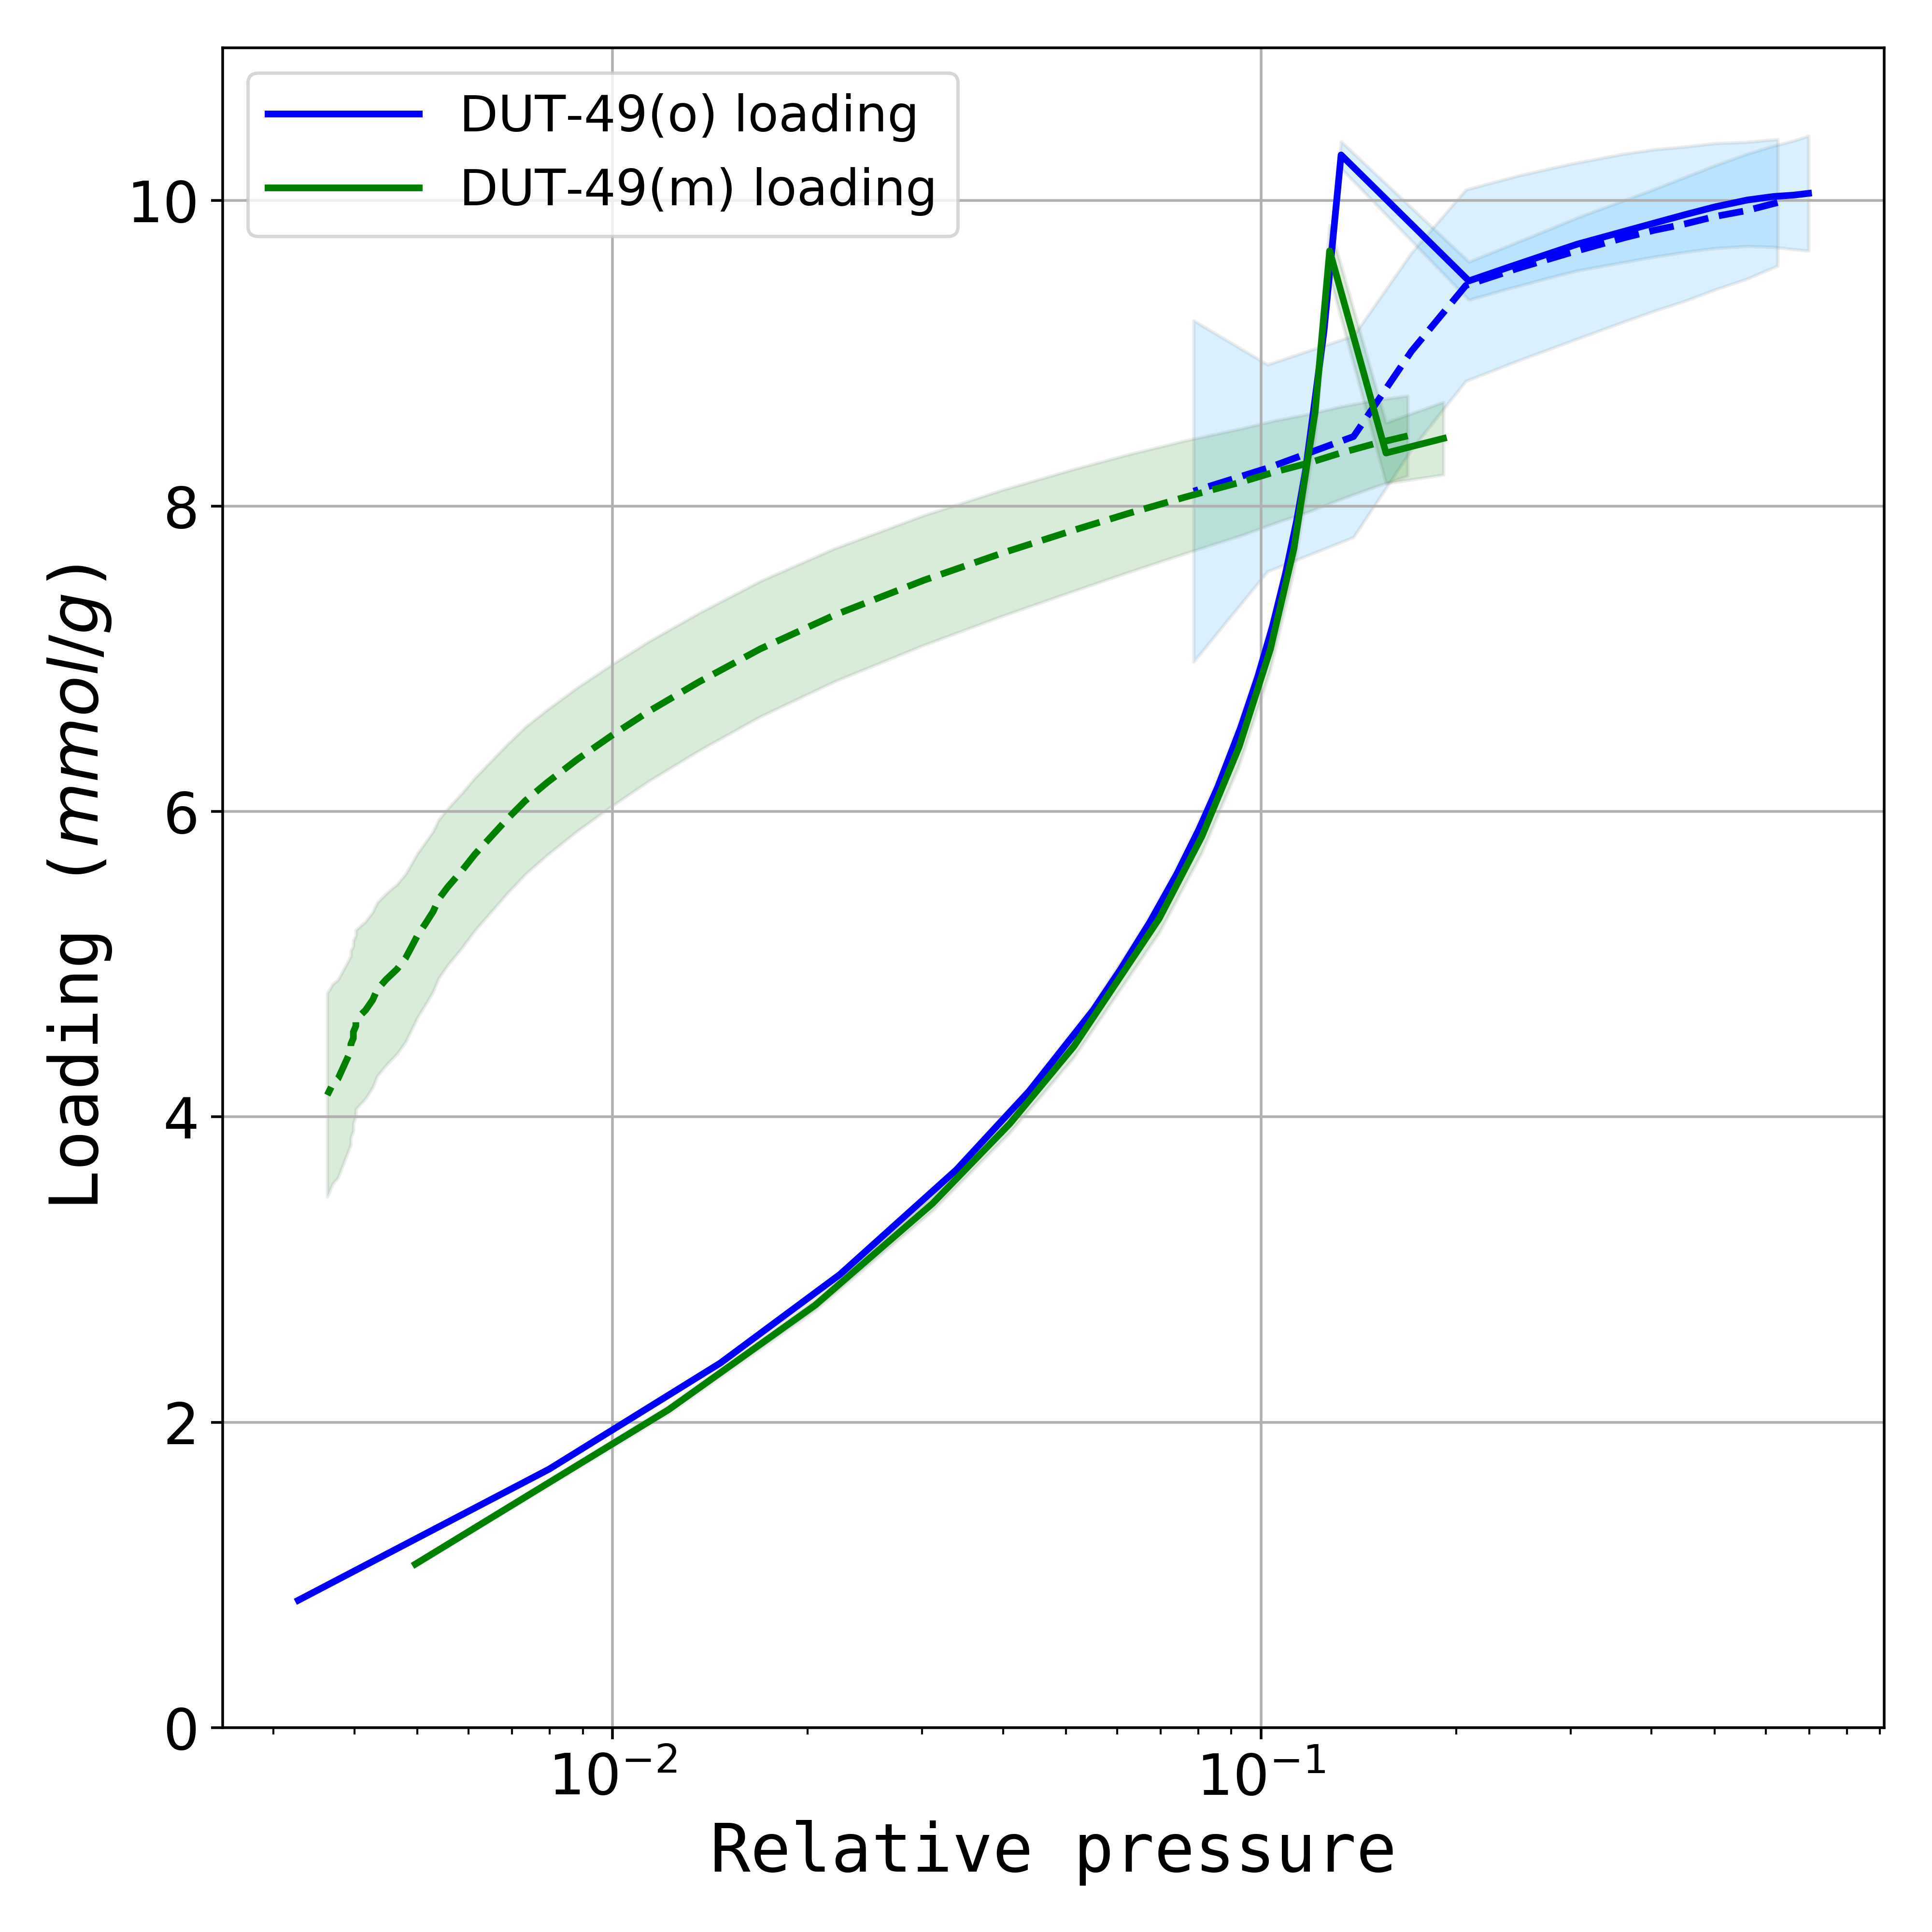
\includegraphics[width=\linewidth]{rtc/dut-49-butane-err-iso}%
        \caption{}\label{dut:fig:dut-49-butane-err-iso}
    \end{subfigure}%
    \begin{subfigure}{0.33\linewidth}
        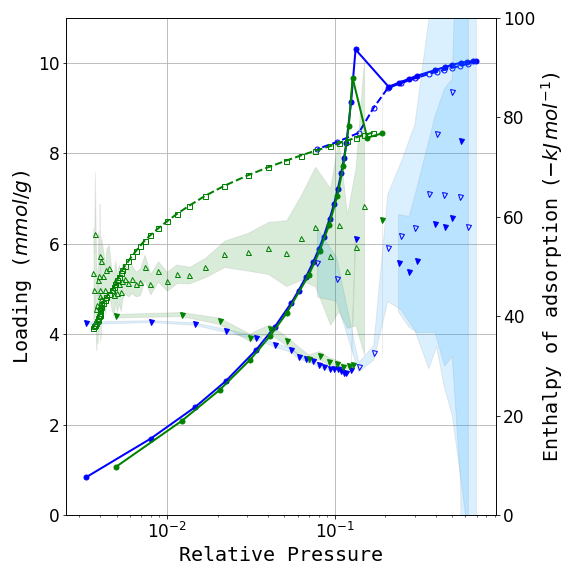
\includegraphics[width=\linewidth]{rtc/dut-49-butane-err-enth}%
        \caption{}\label{dut:fig:dut-49-butane-err-enth}
    \end{subfigure}%
    \begin{subfigure}{0.33\linewidth}
        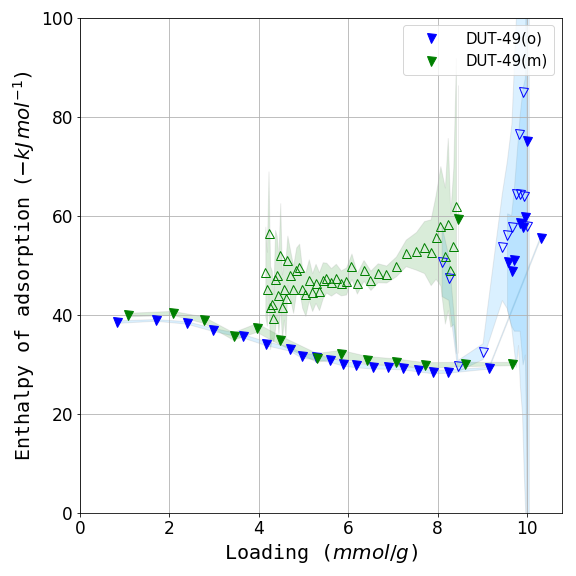
\includegraphics[width=\linewidth]{rtc/dut-49-butane-err-enthp}%
        \caption{}\label{dut:fig:dut-49-butane-err-enthp}
    \end{subfigure}%
    \caption{Estimated errors at a 95\% confidence range for 
    (a) loading as a function of pressure, 
    (b) differential enthalpy as a function of pressure 
    (c) differential enthalpy as a function of loading.}%
    \label{dut:fig:dut-49-butane-err}
\end{figure}

The use of the manometric method for isotherm measurement entails a 
cumulative error in the pressure measurement that leads to an increase
in uncertainty with each measured point. It can be seen in 
\autoref{dut:fig:dut-49-butane-err-iso} that in spite of the margin of 
error, there is perfect overlap between the two measured isotherms
in the adsorption branch and in the desorption branch. It is reasonable
to assume that the error is therefore much smaller than the calculation 
would suggest.

The uncertainty in the differential enthalpy of adsorption 
(\autoref{dut:fig:dut-49-butane-err-enth}) is a 
function of \(\Delta n\), the amount adsorbed in each step, as well
as pressure, with the same cumulative error applicable. The former 
variable accounts for the large uncertainty in flat sections of 
the isotherm where almost no adsorption takes place, while the latter
results in the spread seen at the end of the desorption curves. 
However, when observing \(\Delta_{ads} \dot{h}\) as a function of 
loading in \autoref{dut:fig:dut-49-butane-err-enthp}, the uncertainty 
is confined to high values on the x axis, with a clear separation
of isotherm branches.

As the display of uncertainty ranges clutter the isotherm graphs and 
makes it hard to distinguish features, the remainder of this chapter 
will only display them if the error range is significant.